\chapter{Comportamiento lateral}
\label{ch:lane-change-model}

El problema del cambio de carril determina cuándo y cómo realiza los cambios de carril un conductor en un momento determinado. A priori la intuición sobre el problema es que muchos de los factores determinantes no son medibles en el mundo real y/o en el entorno simulado (e.g. estados de humor, condición física, eventos fortuitos, etcétera).

En un trabajo anterior~\cite{diaz2018modelling} los autores tratamos de controlar muchos de estos factores dividiendo el problema en dos partes, la intención de cambio y la ejecución del cambio, y fijando el primero de tal manera que los conductores sólo cambiaban de carril cuando se les ordenaba. De esta manera se permitía el estudio de cómo diferentes perfiles de conductor ejecutaban de distintas formas los cambios de carril y de cómo este fenómeno es modelable.

En este trabajo se tratará de modelar, sin embargo, el proceso de cambio de carril como un todo, esto es, decidir en cada momento si cambiar a un carril (i.e. izquierda o derecha) o no hacerlo, a partir de las variables medibles del entorno real y simulado. El problema a resolver será, por tanto, de clasificación, donde se tratará de maximizar el número de aciertos entre los cambios de carril realizados y el modelo a ajustar. Las técnicas que se han seleccionado para tratar el cambio de carril son las siguientes:

\begin{enumerate}
	\item \acrshort{mlp}. Los \acrlongplsp{mlp}, más ahora en la época del \textit{deep-learning} son una de las técnicas más usadas para problemas de clasificación. En esta época del \textit{deep-learning} han aumentado su eficiencia varios ordenes de magnitud en capacidad de aprendizaje y, por tanto, en rendimiento a la hora de clasificar.
	\item \acrshort{cnn}. Otro de los grandes exponentes a la hora de clasificar, sobre todo trabajando con mapas de características $n$-dimensionales con las \acrlongplsp{cnn}. Al representar la evolución temporal del entorno circundante como una dimensión más en el espacio presentado a los modelos, podemos aplicar esta técnica para la identificación de características de manera, supuestamente, más eficiente.
\end{enumerate}

Ambos modelos, al igual que con el modelo longitudinal, han sido entrenados ajustando sus parámetros con el algoritmo ADAM \cite{kingma2014adam}. En este caso sin embargo se ha hecho uso de neuronas de activación de tipo \acrshort{relu}\index{ReLU}, salvo en la última capa, donde se ha mantenido el esquema de activación lineal.

El esquema de inicialización de los pesos ha variado también. En un esquema clásico, se basa en valores aleatorios próximos a $0$, donde se encuentra el máximo del gradiente en las funciones de activación sigmoide o tangente hiperbólica. Este mismo esquema, con funciones de activación \acrshort{relu}\index{ReLU}, hace que haya valores negativos y que por tanto existan neuronas no activas desde antes del entrenamiento.

En su lugar, para inicializar los pesos de las variables se hace uso del algoritmo Glorot~\cite{glorot2010understanding}, también denominado Xavier, debido a su mejor funcionamiento en redes con este tipo de funciones de activación. Ésta se basa en intentar mantener la misma desviación típica de gradientes en cada capa de la red. Esta queda determinada en el propio artículo como se expresa en la ecuación~\ref{eq:std-dev-glorot-init}.

\begin{equation}
	\sigma^l = \frac{2}{|W^l_{in}| + |W^l_{out}|}
	\label{eq:std-dev-glorot-init}
\end{equation}

Siendo $|W^l_{in}|$ y $|W^l_{out}|$ el número de entradas y de salidas de la capa, extrayendo posteriormente sus valores de una distribución aleatoria de la forma $X^l \sim \mathcal{N}(\mu=0,\sigma=\sigma^l)$.

Al tratarse además de un problema de clasificación donde las clases son mutuamente excluyentes, a la capa de salida de las redes se le ha aplicado una normalización para transformar el vector de salida en un vector de probabilidades, siendo el cambio de carril seleccionado la salida con el valor de probabilidad más alto. La normalización usada ha sido la operación denominada \textit{softmax}\index{softmax}, definida en la ecuación~\ref{eq:softmax}.
\begin{equation}
	softmax(\vec{x})_i = \frac{e^{x_i}}{\sum_{j=1}^n e^{x_j}}
	\label{eq:softmax}
\end{equation}

Para el cálculo del coste, en lugar de intentar maximizar la cantidad de aciertos (la \textit{precisión}), el error que se ha tratado de minimizar es la entropía cruzada, la cual se trató anteriormente en la sección \ref{ss:mlp} del capítulo \nameref{ch:sota-ci}. Este indicador es mucho más eficiente en problemas de clasificación. Sin embargo, de cara a mostrar resultados, su valor de no ofrece información relevante más allá de \enquote{si decrece es bueno}. Por ellos se ofrecerán los valores de precisión y matrices de confusión que son más acordes con el problema en cuestión.

Antes de pasar a la descripción de los modelos, queda hablar del sesgo existente en los datos de entrenamiento. Debido a la naturaleza el problema, el número de ejemplos existentes de cambios de carril es significativamente menor al existente de no cambios de carril. Este sesgo hace que los modelos se entrenen rápidamente para marcar todos los ejemplos como \enquote{no cambio}, dificultando el ajuste posterior hacia cambios a izquierda o derecha.

Por tanto, debido a que (i) las limitaciones de la máquina no nos permiten operar con los conjuntos completos en cada \textit{epoch} y (ii) existe un sesgo hacia predicciones de \enquote{no cambio}, en cada uno de los \textit{epochs}, se usará un \textit{batch} tamaño $m = 6.000$ compuesto por una selección aleatoria de todos los ejemplos equidistribuidos entre las clases del problema (esto es, aproximadamente $\frac{m}{3}$ para cada clase \enquote{cambio izda.}, \enquote{no cambio} y \enquote{cambio dcha.}).

\section{Descripción de los datasets}

Del conjunto de datos descrito en la Tabla~\ref{tbl:main-variables} (capítulo~\nameref{ch:methodology}) tomaremos aquellos indicadores de interés: \textit{Distancia circulable}, \textit{Distancia a siguiente TLS}, \textit{Estado de siguiente TLS}, \textit{Nube de puntos} y \textit{Cambio de carril}, este último como salida. Estos valores conformarán los conjuntos de entrenamiento y de test tanto para cada uno de los sujetos $S_1$, $S_2$ y $S_3$, como para el conjunto global de éstos $S_A$.

\subsection{Representación de los datos}

Las secuencias de las que se compone el conjunto de datos son, aparte de variables numéricas para cada indicador no espacial, una representación del entorno del vehículo como nube de puntos. Los límites técnicos y la representación en sí implican dos problemas principales:

\begin{enumerate}
	\item Los modelos que utilizamos en esta tesis se basan en un número fijo de entradas. La nube de puntos contiene un número variable de éstos, dependiendo del número de obstáculos.
	\item La nube de puntos se origina a través de un dispositivo mecánico que funciona con coordenadas esféricas a una resolución horizontal de \SI{0.2}{\degree} y vertical de \SI{2}{\degree} con una tasa de refresco de \SI{10}{\hertz}. Esto implica que la superficie del sector circular que no se cubre a largas distancias sea muy extenso, por lo que el espacio según nos alejamos del origen va siendo cada vez más diperso.
\end{enumerate}

Para el primer caso, se ha optado por representar el entorno como un mapa de profundidad, ilustrado en la Figura~\ref{fig:deepmap-example}.

\begin{figure}
	\centering
	
\includegraphics[width=\textwidth]{deepness-map}
	\caption[Mapa de profundidad de ejemplo]{Mapa de profundidad de ejemplo. Un color más oscuro implica más proximidad al obstáculo. La imagen ha sido sometida a un proceso de filtrado gaussiano por motivos de ilustración, pero no se realiza durante los procesos de entrenamiento e inferencia de los modelos.}
	\label{fig:deepmap-example}
\end{figure}

Un mapa de profundidad representa el entorno como una imagen de un sólo canal donde cada píxel representa la distancia a un sector esférico del espacio original. Dado que el \acrshort{lidar}\index{LiDAR} describe el entorno de manera discreta con valores constantes de elevación y azimut\sidenote{
	El \textbf{azimut} se refiere al ángulo de elevación existente desde el suelo.
}, se podría llegar a definir una biyección entre el conjunto de puntos original y los píxeles del mapa de profundidad, por lo que la información disponible en ambas es equivalente. Sin embargo, en nuestro caso no necesitamos una representación tan fiel del entorno porque:

\begin{itemize}
	\item La resolución horizontal produce un mapa de profundidad de $1800$ columnas. Esta resolución es extremadamente grande, y requeriría el uso de modelos con muchos parámetros, pudiendo caer fácilmente en un problema de \textit{over-fitting}.
	\item La apertura vertical del \acrshort{lidar}\index{LiDAR} genera puntos en planos que no son relevantes para el problema. Esto es, planos muy bajos que impactan en el vehículo o muy altos que no impactan con el entorno considerado de interés.
\end{itemize}

Por estas razones, los mapas de profundidad se generarán de una manera más compacta, usando una resolución horizontal de \SI{1}{\degree} y los seis canales que van desde los \SI{-7}{\degree} hasta los \SI{3}{\degree}, lo que nos da un mapa de profundidad con una resolución de $6 \times 360$ con un canal representando la distancia al punto de impacto más cercano contenido en el sector esférico que representa cada posición del mapa.

Para el segundo caso, se ha definido un radio de interés de \SI{25}{\meter}, ya que se ha considerado para el proceso de cambio de carril como un entorno de influencia lo suficientemente amplio para establecer un límite entre información y no relevante para el cambio de carril.

Con estos datos, los mapas de profundidad serán normalizados al intervalo $[0, 1] \in \mathbb{R}$ invertido, esto es, los valores mas cercanos al vehículo serán más próximos a $1$ mientras que los valores más alejados estarán más próximos a $0$.

\subsection{Generación artificial de datos}

Este problema de Los problemas con alta variabilidad de sus entradas suelen ser complejos y requerir de conjuntos de datos de tamaños bastante grandes para poder identificar patrones, como lo son por ejemplo los problemas de reconocimiento de imágenes.

En nuestro caso, el modelo de cambio de carril tiene como entrada una nube de puntos, la cual representa en un espacio de $3$ dimensiones un conjunto muy limitado de puntos, con la dificultad añadida de que el \acrshort{lidar}\index{LiDAR} tiene de base un error de \SI{3}{\cm}. Como el espacio sobre el que trabajar es tan complejo, se requerirían modelos con muchos parámetros, pero al disponer de pocos ejemplos, podríamos caer muy fácilmente en problemas de \textit{over-fitting}.

Por ello, se ha optado por realizar un proceso de generación de datos artificiales a partir de los datos existentes. De esta manera, ayudaremos al modelo a entrenar con casos similares y que de esta manera generalice mejor. La generación artificial se ha realizado sobre los datos recogidos en la ruta $R_1$, ya que es la que nos proporciona la información para entrenar el modelo y es por tanto en el único conjunto que cobra sentido este proceso. Concretamente hemos hecho uso de dos técnicas, primero un \textit{mirroring} sobre todas las filas del conjunto y diez aplicaciones de la técnica \textit{shaking} sobre el nuevo conjunto con los datos originales y simétricos.

La aplicación de estas técnicas requiere además que los nuevos datos generados mantengan una coherencia temporal. Por ello, cada uno se mantendrá en una secuencia independiente.

A continuación se pasan a describir los procesos de generación de datos artificiales introducidos previamente.

\paragraph{mirroring}

Se parte de la suposición de que los procesos cognitivos que producen determinados comportamientos (en nuestro caso, el cambio de carril) son los mismos independientemente de un cambio a la izquierda o hacia la derecha\sidenote{
	Es una suposición que en estudios sucesivos se puede tratar de refutar. Sin embargo, en el estadio actual de la investigación, nos parece razonable asumir que los procesos cognitivos en ambas situaciones son equivalentes.
}.

Por tanto, para cada fila generaremos una nueva nube de puntos a partir de una simetría respecto al plano XY (recordemos que el eje X determina el sentido del movimiento del vehículo). De esta manera, modificando las variables pertinentes\sidenote{
	Es decir, invirtiendo los cambios de carril y la distancia recorrible en carriles izquierdo y derecho.
}, de cada ejemplo obtenemos uno nuevo. En la figura~\ref{fig:mirroring-example} se ilustra un ejemplo de este proceso sobre una nube de puntos arbitraria dentro del conjunto de ejemplos.

\begin{figure}
	\centering
	\subfloat[Original]{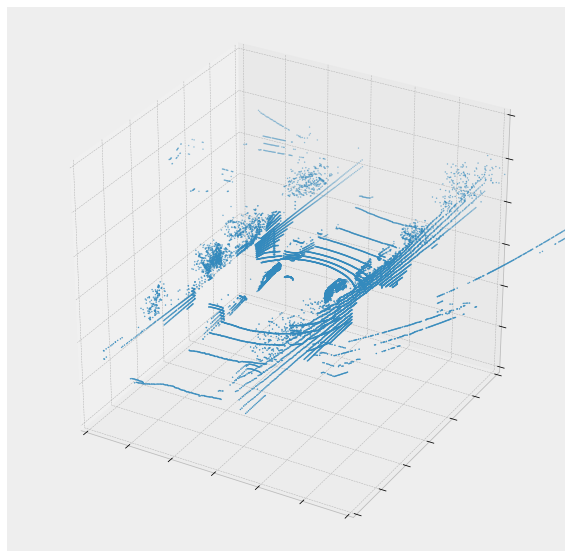
\includegraphics[width=.45\textwidth]{base-pointcloud}}\qquad
	\subfloat[Espejada]{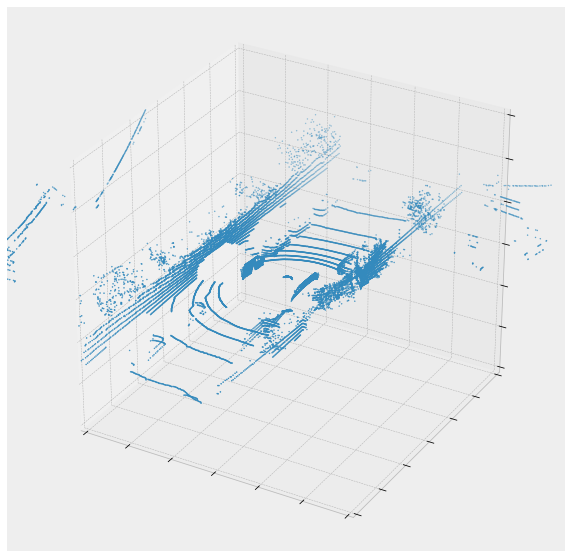
\includegraphics[width=.45\textwidth]{mirrored-pointcloud}}
	\caption[Ejemplo de la técnica de \textit{mirroring}]{Un ejemplo de una nube de puntos (a) original, y (b) tras aplicarle el proceso de mirroring. Para cada fila, tras un proceso de mirroring y una inversión de las variables simétricas en función de la conducción (cambio de carril y distancia recorrible) se genera una nueva fila válida para el conjunto de datos.}
	\label{fig:mirroring-example}
\end{figure}

La principal ventaja de esta aproximación es que es posible doblar el tamaño del conjunto de datos sin añadir más ruido al ya existente.

\paragraph{shaking}

Esta técnica, a diferencia del \textit{mirroring} sí puede llegar a tener impacto en la precisión de los datos. Partiendo siempre de una nube de puntos original, ya que si no los errores entre iteraciones llegarían a hacer la nube ininteligible, se aplica un desplazamiento aleatorio $(\delta x, \delta y, \delta z)$ sobre cada punto tal y como se describe en~\cite{diaz2018modelling}.

La Figura~\ref{fig:shaking-example} ilustra dos procesos de shaking con diferentes desplazamientos sobre la nube original mostrada en la Figura~\ref{fig:mirroring-example}.

\begin{figure}
	\centering
	\subfloat[Shaking $0.05$]{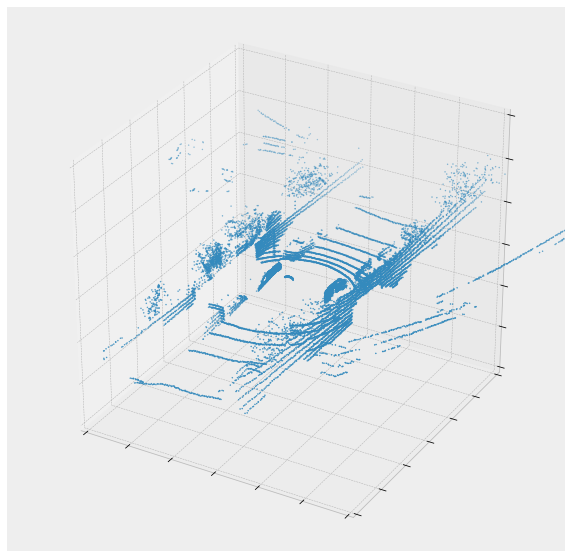
\includegraphics[width=.45\textwidth]{shaken-pointcloud-05}}\qquad
	\subfloat[Shaking $0.2$]{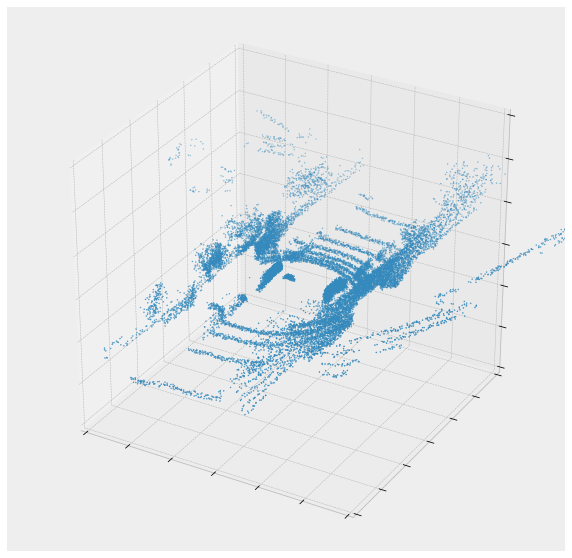
\includegraphics[width=.45\textwidth]{shaken-pointcloud-2}}
	\caption[Ejemplo de la técnica de \textit{shaking}]{Un ejemplo de dos nubes de puntos tras pasar el proceso de shaking con un desplazamiento $(\delta x, \delta y, \delta z)$ de (a) $(0.05, 0.05, 0.05)$ y de (b) $(0.2, 0.2, 0.2)$ sobre la nube de puntos original. Para cada fila, tras un proceso de shaking disponemos de una nueva fila ligeramente diferente de la original, añadiendo ruido y, presumiblemente, generalización al modelo tras el entrenamiento.}
	\label{fig:shaking-example}
\end{figure}

Las especificaciones técnicas del \acrshort{lidar}\index{LiDAR} usado garantizan un error por debajo de los \SI{3}{\cm} de radio, por lo que un desplazamiento aleatorio para cada punto menor o igual que este valor no añadiría más ruido del existente. Sin embargo, en el experimento se ha optado por aplicar un desplazamiento de $\delta x = \delta y = \delta z = 0.05m$ en cada eje, ligeramente superior al proporcionado por el \acrshort{lidar}\index{LiDAR}. De esta forma se pretende la incorporación de ruido sobre el entorno original para aumentar la capacidad de generalización del modelo.

\subsection{Incorporación de información temporal}

Las \ac{cnn} son también redes que funcionan con un esquema \textit{\idx{feed-forward}}, y por tanto tenemos el mismo inconveniente que vimos en el anterior capítulo acerca de mantener una noción temporal en nuestros modelos. En el caso del modelo longitudinal, se consigue este efecto incluyendo variables derivadas de la posición (i.e. velocidad y aceleración). Para el caso del entorno circundante hay que realizar un proceso similar.

Cada una de las filas incluye una representación del entorno en forma de mapa de profundidad, por lo que al modelo le alimentaríamos únicamente con la situación en un instante $t$ de tiempo. Esto no ayuda al modelo a descubrir patrones temporales como la velocidad o la aceleración, ya que no tiene información de eventos anteriores. Para solventar esta limitación, los conjuntos de datos serán transformados en una ventana temporal de parámetros de entrada.

Comenzaremos definiendo el \textit{momento} $t_i$ como aquel ejemplo situado a $t - \frac{i}{10}s$ en el pasado (ver Figura~\ref{fig:moments-illustration}).

\begin{figure}
	\centering
	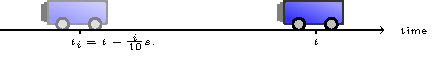
\includegraphics{explanation-of-data-frequency}
	\caption[Momento $t_i$ en el conjunto de datos]{Momento $t_i$ en el conjunto de datos. Un momento $t_i$ se define como el estado en el que se encontraba el vehículo en $t - \frac{i}{10}s$. Por tanto, $t_0$ es el momento actual.}
	\label{fig:moments-illustration}
\end{figure}

Los momentos que se tendrán en cuenta en los datasets finales serán $t_0$, $t_{10}$, $t_{20}$, correspondientes al momento actual, \SI{1}{\second} anterior y \SI{2}{\second} anteriores respectivamente. Estos valores no son arbitrarios, sino que se han elegido de acuerdo a los experimentos realizados en \cite{diaz2018modelling}\sidenote{
	Dichos experimentos trabajan sobre el proceso de ejecución de cambio de carril\index{lane-change}, donde se asume que la maniobra involucra al córtex visual y al córtex prefrontal. Estos procesos cognitivos tienen un tiempo de respuesta de entre \SI{0.2}{\second} y \SI{1.2}{\second}~\cite{buzsaki2012temporal}.
}. Además, incluir tres momentos temporales ayuda a los modelos a intuir patrones correspondientes a la primera y segunda derivadas de la posición (velocidad y aceleración).

Tras este ajuste, los conjuntos de datos están finalizados. Sus propiedades quedan descritas en la Tabla~\ref{tbl:lc-datasets-description}.

\begin{table*}
	\centering
	\caption[Descripción de los conjuntos de datos][2em]{Descripción de los conjuntos de datos para el entrenamiento de los modelos. Los datos de entrenamiento incluyen todos los valores generados tras los procesos de \textit{mirroring} y \textit{shaking}.}
	\label{tbl:lc-datasets-description}
	\begin{tabularx}{\linewidth}{cYYYYYYYY}
		\toprule
		&          &         & \multicolumn{2}{c}{Tamaño}  & \multicolumn{2}{c}{Cambio carril izda.}  & \multicolumn{2}{c}{Cambio carril dcha.}  \\
		& Entradas & Salidas & Entrenamiento & Test & Entrenamiento & Test & Entrenamiento & Test \\
		\midrule
		\rowcolor{black!20} $LC_{S_1}$ & $8653$ & $3$ & $68990$  & $2057$ & $820$  & $43$  & $820$  & $13$  \\
		$LC_{S_2}$ & $8653$ & $3$ & $84810$  & $2886$ & $925$  & $27$ & $925$  & $17$  \\
		\rowcolor{black!20} $LC_{S_3}$ & $8653$ & $3$ & $82060$  & $2890$ & $995$  & $51$  & $995$  & $23$ \\
		$LC_{S_A}$ & $8653$ & $3$ & $248930$ & $7833$ & $2740$ & $121$ & $2740$ & $53$ \\
		\bottomrule
	\end{tabularx}
\end{table*}

\section{Modelo basado en \acrlongplsp{mlp}\index{perceptron multicapa}}

Los entrenamientos han sido realizados sobre diferentes topologías, siendo las más representativas las descritas en la tabla~\ref{tbl:lc-mlp-architectures}.

\begin{table*}
	\centering
	\caption[Resumen de las arquitecturas \acrshort{mlp} para el modelo de cambio de carril][1.8em]{Resumen de las arquitecturas de \acrlongplsp{mlp} para el modelo de cambio de carril. La posición de cada número de la topología indica la capa, siendo su valor el número de nodos (neuronas) que incluye dicha capa. Las arquitecturas seleccionadas en esta tabla son aquellas consideradas relevantes tras un proceso manual de ensayo y error.}
	\label{tbl:lc-mlp-architectures}
	\begin{tabularx}{\linewidth}{cYYYYY}
		\toprule
		\multirow{2}{*}{} & \multirow{2}{*}{Topología} & \multirow{2}{*}{Epochs} & \multicolumn{3}{c}{Precisión} \\
		& & & Entrenamiento & Validación & Test \\
		\midrule
		\rowcolor{black!20} $MLP_1$ & $64, 64$ & $10^5$ & $0.33$ & $0.33$ & $0.33$ \\
		$MLP_2$ & $1024, 512, 128$  & $10^5$ & $0.33$ & $0.33$ & $0.33$ \\
		\rowcolor{black!20} $MLP_3$ & $1024, 512, 256, 128$ & $10^5$ & $0.33$ & $0.33$ & $0.33$ \\
		\bottomrule
	\end{tabularx}
\end{table*}

La tasa de \textit{dropout} utilizada en estos experimentos es de $0.1$, es decir, en cada \textit{epoch} mantenemos activas un $90\%$ de las neuronas existentes en toda la arquitectura.

La Figura~\ref{fig:lc-mlp-accuracy-comparison} nos muestra la evolución de la precisión alcanzada por los modelos a lo largo del entrenamiento, tanto en entrenamiento como en el posterior test.

\begin{figure}
	\centering
	\subfloat[Entrenamiento y validación]{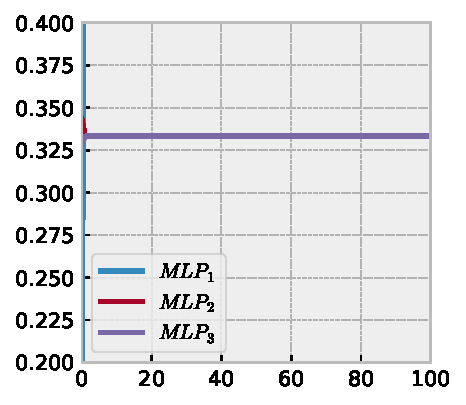
\includegraphics[width=.45\textwidth]{lc-mlp-acc-all-training-and-validation-detail}}\qquad
	\subfloat[Test]{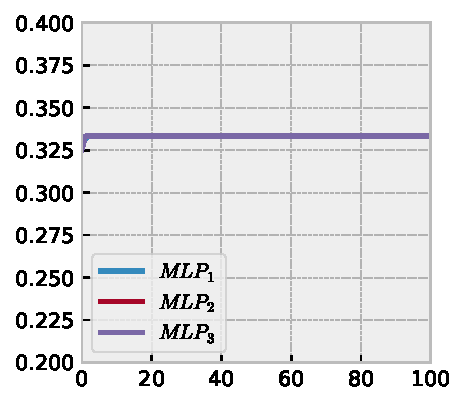
\includegraphics[width=.45\textwidth]{lc-mlp-acc-all-test-detail}}
	\caption[Comparación de las precisiones alcanzadas por los modelos de tipo \acrshort{mlp}]{Comparación de las precisiones alcanzadas por los modelos de tipo \acrlongsp{mlp}.}
	\label{fig:lc-mlp-accuracy-comparison}
\end{figure}

Cada una de las redes se ha entrenado durante $10^5$ epochs. Los resultados indican que la capacidad de predicción de este tipo de redes con el conjunto de datos propuesto no supera el valor de predecir de forma aleatoria. Además, en  ningún caso las redes desarrolladas han sido capaces de superar ese valor (sí el caso del entrenamiento). Por tanto, el uso de \acrlongplsp{mlp}\index{perceptron multicapa} aquí es descartado definitivamente.

\section{Modelo basado en \acrlongplsp{cnn}\index{red de convolución}}

Las arquitecturas de los modelos que mejores resultado han arrojado tras las pruebas se describen en la Tabla~\ref{tbl:lc-cnn-architectures}. La tasa de \textit{dropout} utilizada en los entrenamientos ha sido de $0.1$.

\begin{table*}
	\centering
	\caption[Resumen de las arquitecturas \acrshort{cnn} para el modelo de cambio de carril][2em]{Resumen de las arquitecturas de \acrlongplsp{cnn} para el modelo de cambio de carril. La posición de cada número de la topología indica la capa, siendo su valor el número de nodos (neuronas) que incluye dicha capa. Las arquitecturas seleccionadas en esta tabla son aquellas consideradas relevantes tras un proceso manual de ensayo y error.}
	\label{tbl:lc-cnn-architectures}
	\begin{tabularx}{\linewidth}{ccYYYY}
		\toprule
		\multirow{2}{*}{} & \multirow{2}{*}{Topología} & \multirow{2}{*}{Epochs} & \multicolumn{3}{c}{Precisión} \\
		& & & Entrenamiento & Validación & Test \\
		\midrule
		\rowcolor{black!20} $CNN_1$ & c16-4-18-v d128 & $10^5$ & $0.589$ & $0.576$ & $0.573$ \\
		$CNN_2$ & c64-5-36-v c256-3-5-v d256-d128-d16                       & $10^6$ & $0.506$ & $0.531$ & $0.518$ \\
		\rowcolor{black!20} $CNN_3$ & c16-3-18-v c32-3-18-v c64-2-18-v d128 & $10^6$ & $0.561$ & $0.569$ & $0.554$ \\
		\bottomrule
	\end{tabularx}
\end{table*}

La descripción de los parámetros de las arquitecturas es la siguiente:

\begin{itemize}
	\item \textbf{$cF$-$W$-$H$-$x$}. Esta nomenclatura se corresponde con una capa de convolución de $F$ filtros donde cada uno tiene un tamaño de $W \times H$. $x$ puede tomar el valor $v$ (de \textit{valid}) o $s$ (de \textit{same}), dependiendo de si se desea que el filtro se limite a las dimensiones de la entrada o si por el contrario se prefiere que sobrepase los límites para que las convoluciones den como resultado una salida del mismo tamaño que la entrada original, respectivamente.
	\item \textbf{$dN$-$r$}. Esta capa se corresponde con las capas \textit{fully-connected} que trabajan sobre el espacio de las características extraídas en las convoluciones. En esta nomenclatura, $N$ se corresponde con el número de neuronas que tiene la capa y $r$ con la tasa de \textit{dropout} aplicada a sus neuronas.
\end{itemize}

Existen una serie de particularidades del proceso de entrenamiento que hay que destacar. La primera y principal es la modificación de la arquitectura básica de una \ac{cnn} para atender a variables que no obedecen al esquema de mapa $n$-dimensional. Una \ac{cnn} basa su funcionamiento en una fase de extracción de características seguida de una fase de inferencia sobre las características extraídas de la imagen. En nuestro caso, sin embargo, necesitamos alimentar a la red con más información.

La decisión tomada ha sido entender estas variables (\textit{Distancia circulable}, \textit{Distancia a siguiente TLS} y \textit{Estado de siguiente TLS}) como características del modelo ya extraídas. Para ello, al alimentar el modelo, los mapas de profundidad y estas variables son separadas al comenzar el entrenamiento. Los mapas de profundidad se pasan por el flujo normal de funcionamiento y una vez se han extraído las características de estos mapas se combinan con las variables para continuar con el flujo normal (ver Figura~\ref{fig:modification-of-cnn-to-work-with-variables})

\begin{figure}
	\centering
	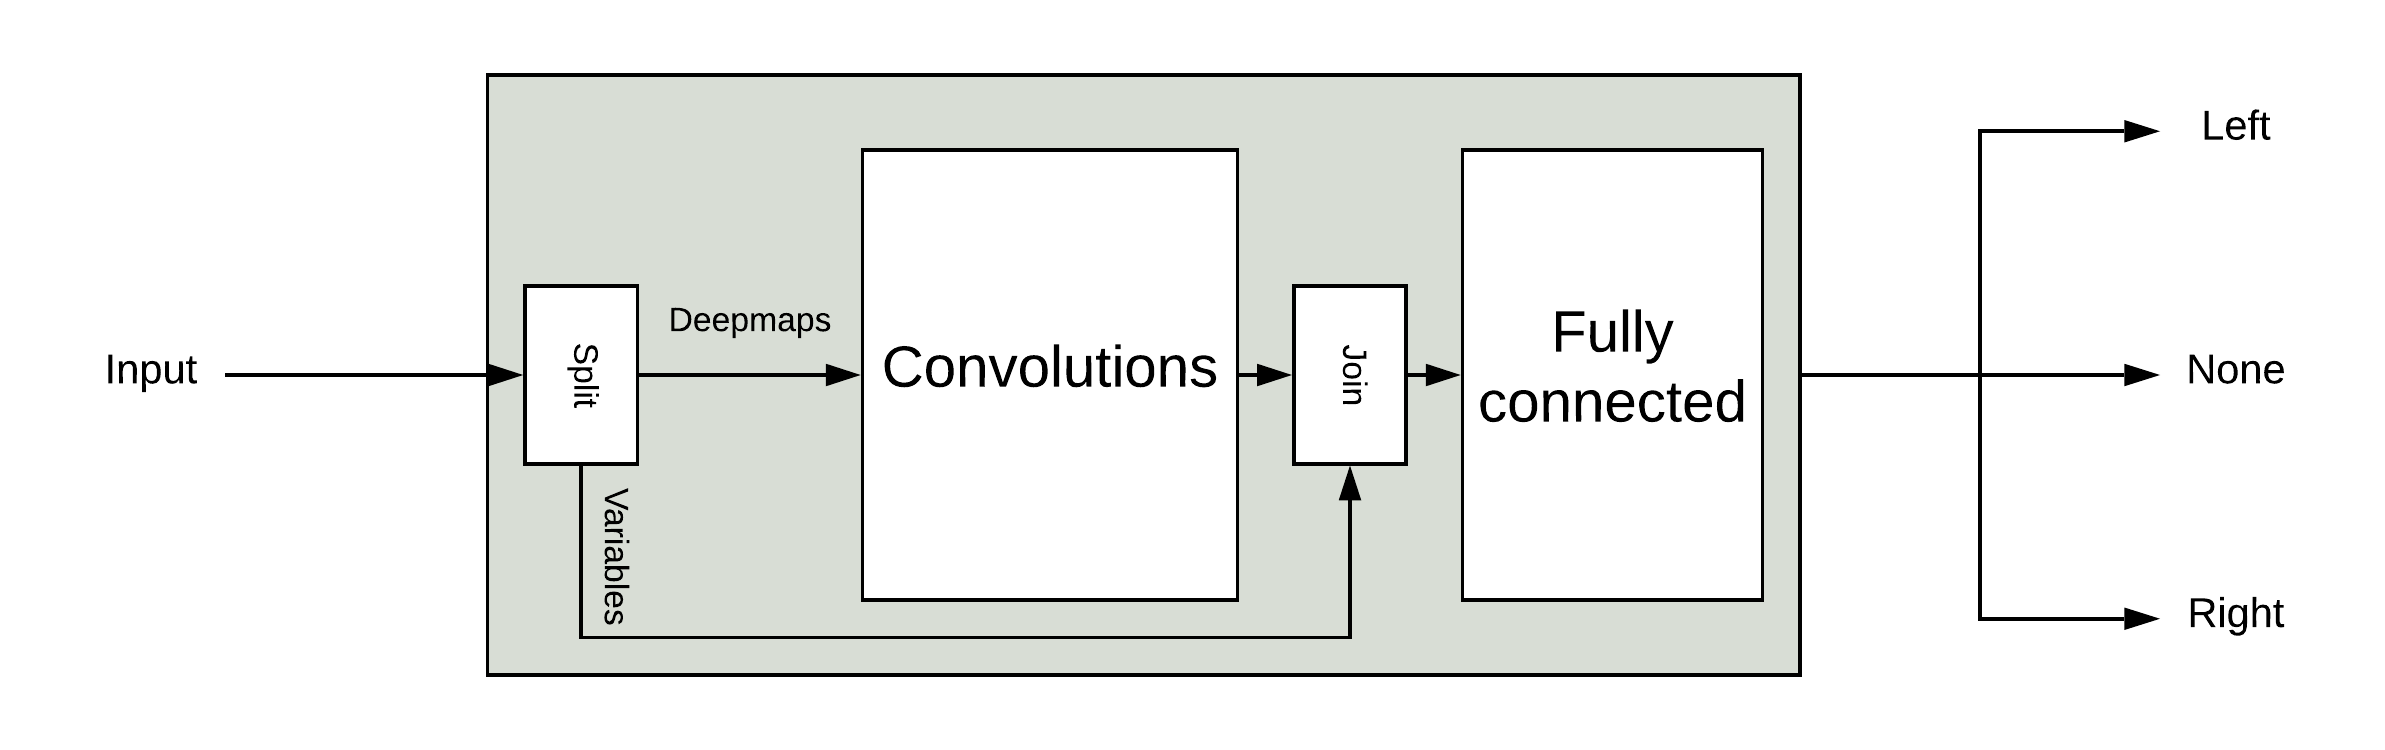
\includegraphics{modification-of-cnn-to-work-with-variables}
	\caption[Esquema de modificación de \acrshortpl{cnn} para incluir características no espaciales]{Esquema de modificación de \acrlongsp{cnn} para incluir características no espaciales. Las variables se separan al principio de la convolución para que éstas trabajen con las imágenes. Una vez este proceso se ha completado, las características de las imágenes y las variables de entrada separada se vuelven a continuar para continuar el flujo normal de funcionamiento.}
	\label{fig:modification-of-cnn-to-work-with-variables}
\end{figure}

La siguiente modificación ha sido la alteración del mapa de profundidad justo al comienzo de la alimentación. Al ser los mapas de profundidad una representación cilíndrica de las distancias, el extremo izquierdo y el derecho de la imagen son, en realidad, un punto de corte donde las convoluciones perderán información. Para evitar esta limitación, las imágenes con las que se alimenta la red son aumentadas artificialmente en sus bordes con el extremo contrario de la imagen (ver Figura~\ref{fig:deepmap-augmentation-in-cnn}), para que la convolución opere sobre la información que de otro modo se perdería.

\begin{figure}
	\centering
	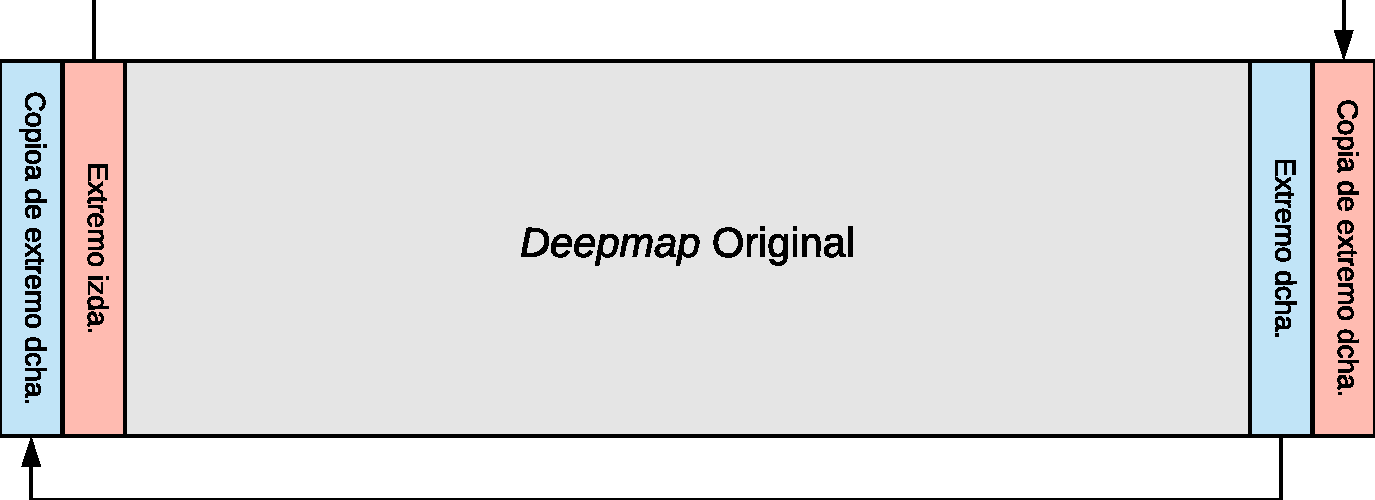
\includegraphics{deepmap-augmentation-in-cnn}
	\caption[\textit{Padding} artificial en los extremos del mapa de profundidad]{\textit{Padding} artificial en los extremos del mapa de profundidad. Para no perder información que puede ser relevante, los mapas se aumentan artificialmente al alimentar a la red, de tal manera que a los extremos izquierdo y derecho se les aumenta con parte de los extremos derecho e izquierdo con un número de píxeles igual a la mitad del tamaño horizontal del los filtros que los recorrerán.}
	\label{fig:deepmap-augmentation-in-cnn}
\end{figure}

La última modificación es la de la aplicación de una tasa de aprendizaje adaptativa al proceso de entrenamiento. Esta adaptación puede basarse en muchos factores, pero en nuestro caso la tasa se basa en una disminución suave de un valor máximo a un valor mínimo de manera que en los primeros estadios del entrenamiento la tasa sea suficientemente alta como para converger rápidamente a zonas de interés, pero que a la vez, según el entrenamiento avanza, se eviten los problemas de saltos alrededor de mínimos. La tasa de aprendizaje en cada \textit{epoch} quedará determinada por la siguiente ecuación:

\begin{equation}
    \alpha_i = \alpha_{min} + (\alpha_{max} - \alpha_{min}) \cdot e^\frac{i}{\alpha_d}
	\label{eq:learning-rate-decay}
\end{equation}

Donde $\alpha_i$ será la tasa de aprendizaje a aplicar en el \textit{epoch} $i$, $\alpha_{min}$ y $\alpha_{max}$ las cotas inferior y superior que tomará la tasa de aprendizaje y $\alpha_d$ la tasa de decrecimiento. En la Figura~\ref{fig:learning-rate-decay} se ilustra la gráfica de la función usada para entrenar las arquitecturas de esta sección.

\begin{figure}
	\centering
	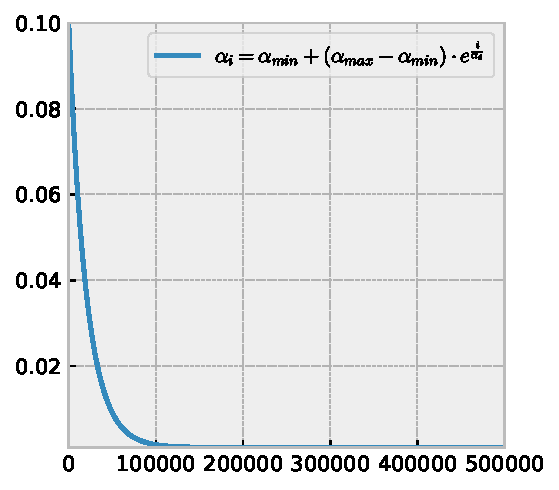
\includegraphics[width=6cm]{lc-learning-rate-decay}
	\caption[Gráfica de la tasa de aprendizaje adaptativo por \textit{epoch} usada para entrenar \acrshortpl{cnn}]{Gráfica de la tasa de aprendizaje adaptativo por epoch usada para entrenar \acrlongplsp{cnn}. En nuestros entrenamientos, los valores de los parámetros son $\alpha_{min} = 0.1$ y $\alpha_{max} = 0.001$ y $\alpha_d = 20000$.}
	\label{fig:learning-rate-decay}
\end{figure}

Un último apunte antes de pasar a mostrar las gráficas de los entrenamientos. No se ha incluido ninguna capa de \textit{pooling} en las arquitecturas, sino que se ha preferido usar las capas de convolución sin añadir padding para ese efecto, tal y como proponen en~\cite{howard2017mobilenets}.

La evolución de la precisión a lo largo del entrenamiento para las diferentes arquitecturas se muestra en la Figura~\ref{fig:lc-cnn-training-validation-test-comparison}.

\begin{figure}
	\centering
	\subfloat[Entrenamiento y validación]{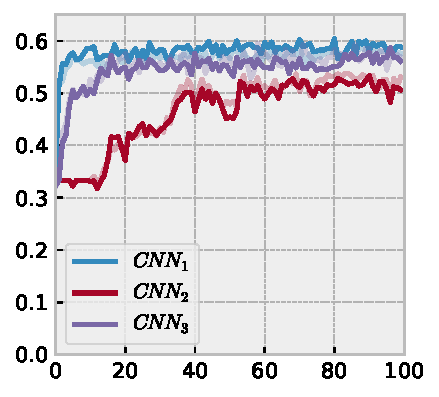
\includegraphics[width=.45\textwidth]{lc-cnn-acc-all-training-and-validation-detail}}\qquad
	\subfloat[Test]{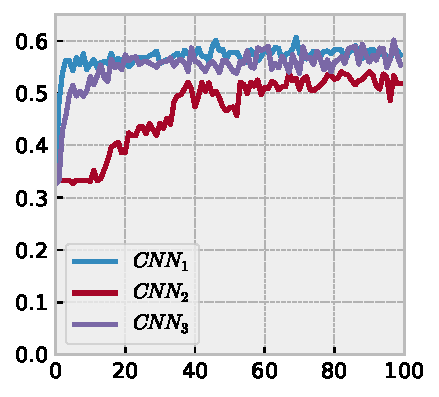
\includegraphics[width=.45\textwidth]{lc-cnn-acc-all-test-detail}}
	\caption[Comparación de las precisiones alcanzadas por los modelos de tipo \acrlongsp{cnn}]{Comparación de las precisiones alcanzadas por los modelos de tipo \acrshort{cnn}.}
	\label{fig:lc-cnn-training-validation-test-comparison}
\end{figure}

Se puede observar que se ha necesitado una red relativamente grande para superar el límite impuesto por la clasificación aleatoria. Esto contrasta con los resultados obtenidos en~\cite{diaz2018modelling}, donde los valores de clasificación eran mucho más altos. La razón por la que se intuye esta disparidad de datos es que es precisamente la operación de \textbf{decisión de cambio de carril} la que es más compleja de modelar, a diferencia de la de \textbf{ejecución de cambio de carril}, en la que esta decisión está ya tomada.

Probablemente con otra serie de variables se pueda aumentar la precisión de estos modelos, pero en este experimento estamos limitados al conjunto de variables observables en los entornos real y de simulación.

\section{Comparación entre modelos}

En este caso, de las dos técnicas propuestas para los modelos, los \acrlongplsp{mlp}\index{perceptron multicapa} ha sido descartados completamente al ser sus clasificaciones iguales a la de la selección aleatoria. Por tanto, el modelo que usaremos será el $CNN_2$, ya que es la única arquitectura que supera este límite.

En la figura~\ref{fig:lc-cnn-model-confussion-matrix} se expone la matriz de confusión asociada a esta arquitectura para los valores existentes en el conjunto de test.

\begin{figure}
	\centering
	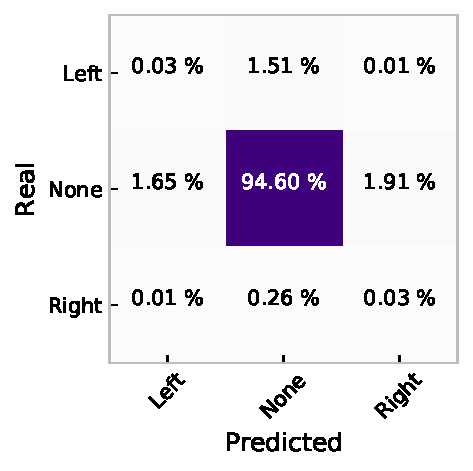
\includegraphics[width=.6\linewidth]{lc-cnn-model-confussion-matrix}
	\caption[Matriz de confusión del conjunto de test para el modelo de cambio de carril seleccionado]{Matriz de confusión del conjunto de test para el modelo de cambio de carril seleccionado.}
	\label{fig:lc-cnn-model-confussion-matrix}
\end{figure}

\section{Modelos laterales específicos}

Como indicamos en el capítulo \nameref{ch:longitudinal-model}, se generarán los modelos de cada uno de los conductores por separado. 
En la Figura~\ref{fig:lc-specific-rmse-all-test-detail} se muestra la evolución del \gls{rmse}\index{RMSE} en test para cada uno de los sujetos tras entrenar los modelos de arquitectura $CNN_2$ con los datos de los sujetos.

\begin{figure}
	\centering
	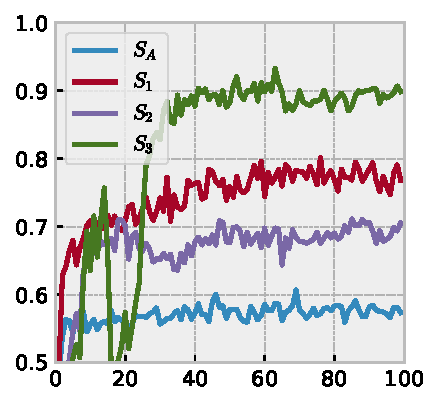
\includegraphics[width=\textwidth]{lc-specific-rmse-all-test-detail}
	\caption[\gls{rmse} en test entre los sujetos de la arquitectura seleccionada para el modelo de cambio de carril]{Comparativa de la evolución de la precisión en test entre los sujetos de la arquitectura seleccionada para el modelo de cambio de carril.}
	\label{fig:lc-specific-rmse-all-test-detail}
\end{figure}

La precisión alcanzada en los modelos específicos entrenados con esta arquitectura es mayor que la alcanzada por el modelo global. Tiene sentido ya que el modelo global se ha entrenado con el conjunto de datos global y por tanto no obedece exactamente al comportamiento de ningún perfil en concreto, mientras que en los modelos específicos sí. En la Tabla~\ref{tbl:lc-specific-accuracy} se exponen los valores de la precisión de este modelo.

\begin{table}
	\centering
	\caption[Precisión alcanzada para los modelos específicos de cambio de carril]{Resumen de los valores de precisión para los modelos específicos de cambio de carril.}
	\label{tbl:lc-specific-accuracy}
	\begin{tabularx}{\linewidth}{cYYY}
		\toprule
		\multirow{2}{*}{} & \multicolumn{3}{c}{\ac{rmse}}      \\ 
		& Entrenamiento & Validación & Test \\
		\midrule
		\rowcolor{black!20} $S_A$ & $0.588$ & $0.576$ & $0.573$  \\
		$S_1$ & $0.805$ & $0.763$ & $0.768$  \\
		\rowcolor{black!20} $S_2$ & $0.683$ & $0.708$ & $0.706$  \\
		$S_3$ & $0.727$ & $0.706$ & $0.710$  \\
		\bottomrule
	\end{tabularx}
\end{table}

Para comprobar que esta topología es capaz de capturar las diferencias entre cómo cambian de carril los conductores, compararemos las tasas de acierto en sus respectivos conjuntos de test. La Tabla~\ref{tbl:lc-subjects-comparison} muestra los índices de precisión de los sujetos sobre cada uno de los conjuntos de test de los demás.

\begin{table}
	\centering
	\caption[Comparación de la precisión para los diferentes modelos de cambio de carril]{Comparación de la precisión para los diferentes modelos de cambio de carril. Las filas se corresponden con los recorridos mientras que las columnas se corresponden con los modelos que se han intentado ajustar a ellas.}
	\label{tbl:lc-subjects-comparison}
	\begin{tabularx}{\linewidth}{cYYY}
		\toprule
		& $S_1$ & $S_2$ & $S_3$ \\
		\midrule
		\rowcolor{black!20} $S_1$ & $0.768$ & $0.314$ & $0.601$ \\
		$S_2$ & $0.601$ & $0.706$ & $0.511$ \\
		\rowcolor{black!20} $S_3$ & $0.648$ & $0.666$ & $0.710$ \\
		\bottomrule
	\end{tabularx}
\end{table}


 basados en la arquitectura $CNN_2$ representarán el control lateral de los sujetos en el simulador. Veremos su desempeño en el capítulo \nameref{ch:simulation-implementation}.
